\documentclass[12pt]{notes}

% Command for Questions
%\question{}

% Command for Notes
% \note{}

% Code to create a minipage where you can type in class notes. 
%%\begin{minipage}[l][2cm][c]{\textwidth}
\begin{comment}

\end{comment}
%%\end{minipage}


% Begin Document
%==============================================================================
\begin{document}
% Include the Title of the Handout
\ntitle{2.5: Multiple Linear Regression}

% Include Numbered Sections
\section{Why Multiple Linear Regression?}
\bi
\item Models that use a single explanatory variable to predict a response are very limited in terms of its capability. 
\item We are often interested in determining the effect of an explanatory variable on the response variable \textit{after} accounting for the effects due to other explanatory variables. 
\bi
\item Example: Is there a difference in the pay based on gender after accounting for job type and hours worked? 
\ei
\ei

\nspace
\question{(Individual) Can you think of another scenario where using multiple predictors would be useful in predicting a single response variable? }

\begin{minipage}[l][3cm][c]{\textwidth}
\begin{comment}
\note{Potential Example: Use lot size, lot type, square footage, elevation, to predict house price in Cache County, Utah.}
\end{comment}
\end{minipage}


\section{What Changes from Simple Linear Regression?}
\begin{enumerate}
\item Interpretation of coefficients
\begin{eqnarray}
  Y_i & = & \beta_0 + \beta_1 X_{i1} + \beta_2 X_{i2} + \ldots + \beta_{p-1} X_{i,p-1} + \varepsilon_i \nonumber \\
   & & \nonumber \\
\beta_0 & = & E[Y | X_1=X_2=\cdots=X_{p-1}=0] \nonumber \\
& & \nonumber \\
\beta_k & = & \mbox{expected (or average) change in Y} \nonumber \\
  & & \mbox{for every unit increase in predictor $X_k$,}\nonumber\\
  & & \mbox{\underline{while holding all other predictors constant}}\nonumber
\end{eqnarray}

\begin{minipage}[l][1cm][c]{\textwidth}
\begin{comment}
\note{Need all three elements for a correct interpretation.}
\end{comment}
\end{minipage}

$\beta_k$ sometimes called ``partial regression coefficient''
because it reflects partial effect of $X_k$ on $Y$ \underline{after
accounting for effects of other predictors}\\

\item ANOVA table
\begin{itemize}
  \item model $df = p-1$ = \# of predictor variables
  \item error $df = n-p$\\
        -- we have to ``spend'' more degrees of freedom to calculate the additional coefficients
  \item model F-test more meaningful:
        \begin{eqnarray}
          H_0 & : & \beta_1 = \beta_2 = \ldots = \beta_{p-1} = 0   \nonumber \\
          H_a & : & \beta_k \neq 0 \mbox{ for at least one } k=1,\ldots,p-1 \nonumber
        \end{eqnarray}
  \item $R^2$ called coefficient of multiple determination (still interpret as \% variance in $Y$ explained by model);
        $\sqrt{R^2}$ called coeff. of multiple correlation
\end{itemize}

\item Refer to regression ``surface'' instead of ``line''\\ 

\begin{figure}[H]
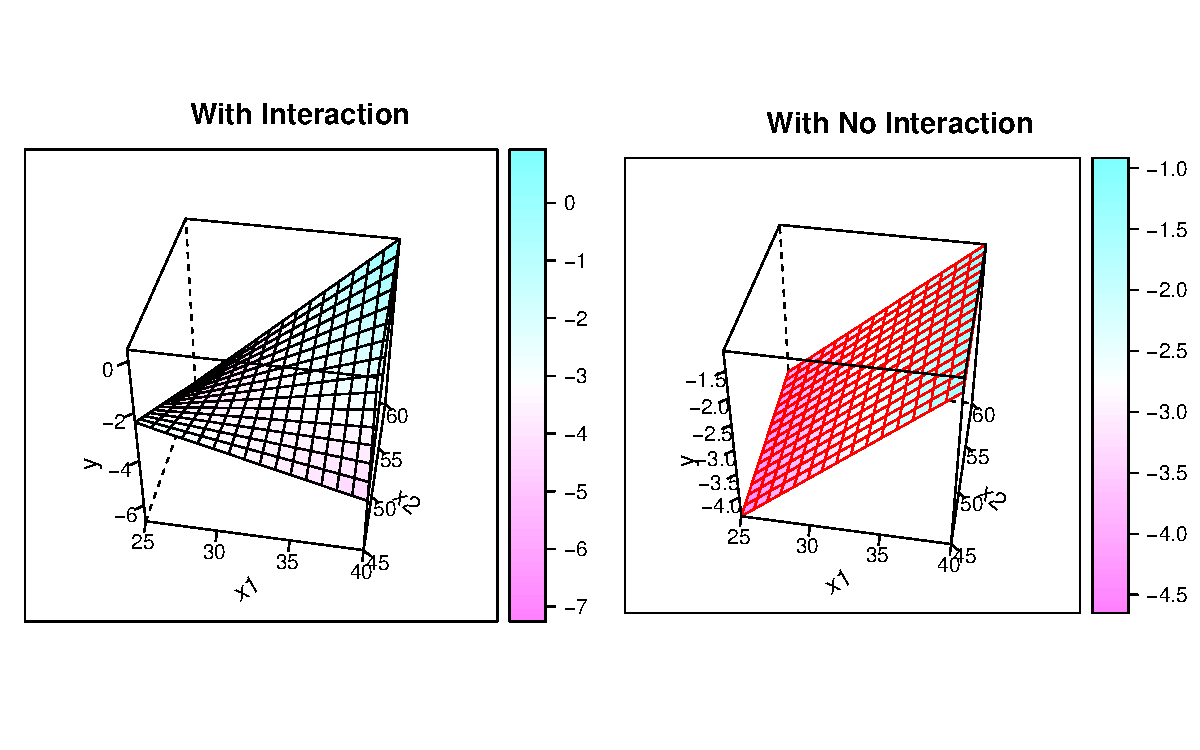
\includegraphics[width = \textwidth, trim = 0cm 1cm 0cm 1cm, clip]{figures/module2/surface.pdf}
\caption{Regression surface using two X variables to predict Y. Harder to visualize when there are more than two predictor variables.}
\end{figure}

\item F-test for lack of fit less practical
\begin{itemize}
  \item requires multiple observations at one or more X profiles, which is hard to achieve when the number of X's is large. 
  \item ``X-profile'' or ``covariate profile'' refers to specific values for all predictors
\end{itemize}

\item More assumptions to check later -- regarding inter-related predictors
\begin{itemize}
 \item basically, if predictors are related to each other, the model becomes very hard to interpret
\end{itemize}

\item Other variable types can be included\\
(interactions, qualitative, higher-order) -- (more in Module 3)\\


\end{enumerate}

\newpage

\section{Matrix Approach to Multiple Linear Regression}

When the number of X variables gets large, the matrix representation of linear regression models is easier to write and understand. 


\begin{eqnarray}
  Y & = & (Y_1, \ldots, Y_n)'  =  \mbox{vector of response variable} \nonumber \\
   & \nonumber \\
  \varepsilon & = & (\varepsilon_1, \ldots, \varepsilon_n)'  =  \mbox{vector of error terms}  \nonumber \\
   & \nonumber \\
  X_k & = & (X_{1k}, \ldots, X_{nk})'  =  \mbox{vector of predictor variable \#k \hspace{1em}}(k=1,\ldots,p-1) \nonumber \\
   & \nonumber \\
  X & = & [\mbox{\hspace{1em}} 1 \mbox{\hspace{1em}} X_1 \mbox{\hspace{1em}} \ldots \mbox{\hspace{1em}} X_{p-1} \mbox{\hspace{1em}} ] 
      = \mbox{matrix with $p$ columns and $n$ rows} \nonumber \\
   & \nonumber \\
  \beta & = & (\beta_0, \beta_1, \ldots, \beta_{p-1})'  = \mbox{vector of coefficients} \nonumber \\
     & \nonumber \\
  b & = & (b_0, b_1, \ldots, b_{p-1})'  = \mbox{vector of coefficient \underline{estimates}} \nonumber \\
   & \nonumber
\end{eqnarray}

Then regression model is
\begin{eqnarray}
  Y & = & X \beta + \varepsilon \nonumber \\
    & \nonumber \\
  \varepsilon & \sim & N(0,\sigma^2 I) \nonumber \\
    & \nonumber
\end{eqnarray}

\vspace{-3.5em}
\begin{tabular}{l l}
\hspace{25em} &
\begin{minipage}[t]{2in}
 $I$ = ``identity'' matrix
\end{minipage}
\end{tabular}

Estimates:
\begin{eqnarray}
  b & = & (X' X)^{-1} X' Y \nonumber \\
   & \nonumber \\
  \mbox{truth: \hspace{1em}} Cov(b) & = & (X' X)^{-1} \sigma^2 \nonumber \\
  \mbox{estimated: \hspace{1em}}  s^2 \{ b \} & = & (X' X)^{-1} \cdot \mbox{MSE} \nonumber \\
   & \nonumber
\end{eqnarray}

\vspace{-8.5em}
\begin{tabular}{l l}
\hspace{30em} &
\begin{minipage}[t]{2in}
 Matrices with variance on diag., covariance on off-diag.
\end{minipage}
\end{tabular}

\vspace{2.75em}
\begin{tabular}{l l}
\hspace{32em} &
\begin{minipage}[t]{2in}
 $\sqrt{\mbox{diag. elements}}$ gives\\ SE's of $b_k$'s
\end{minipage}
\end{tabular}

\vspace{1em}

We'll come back to this, but for now, note that
\begin{eqnarray}
  \hat{Y} & = & X b \nonumber \\
          & = & X (X' X)^{-1} X' Y \nonumber \\
          & \nonumber \\
          & = & H Y \nonumber \\
          & \nonumber
\end{eqnarray}

H projects Y down to column space of X:\\

\begin{minipage}[t]{4in}
  \begin{itemize}
    \item $Y$ = observed response values vector; \underline{is not}\\ a [perfect] linear combination of predictor variables
    \item $\hat{Y}$ = predicted response values vector; \underline{is}\\ a [perfect] linear combination of predictor variables
  \end{itemize}
\end{minipage}













% End the Document
%==============================================================================
\end{document}